%! TEX root = ../main.tex
\section{Interfaz de Usuario}
\label{sec:res_INTERFAZ}

Previamente a las pruebas realizadas con la población objetivo y durante el
desarrollo de la solución se realiza la prueba de interfaz para encontrar
problemas en la misma que puedan impedir su fácil uso por los usuarios finales.
Posterior a la prueba se realizaron modificaciones para la mejora de la misma
según los resultados que se presentan a continuación.

Como fue descripta en la sección~\ref{sec:interfaz} la encuesta realizada a cada
usuario, parte de la prueba, es utilizada para obtener el grado de
disconformidad de los mismos. Las preguntas que forman parte de la  encuesta son
agrupadas en cuanto a aspectos de calidad gráfica, interacción con el entorno,
interacción con los objetos, características del entorno, usabilidad de la
interfaz e integración con el hardware.

Luego de estas agrupaciones obtenemos el resultado que se muestra en la
tabla~\ref{tab:interfaz_disconformidad_metrica}. En esta tabla se puede observar
que las mayores disconformidades son con respecto a la usabilidad de la interfaz
que llega al $51\%$, la interacción de los usuarios con el entorno que llega al
$50\%$, la interacción con los objetos que llega al $49\%$. Luego, se pueden
observar también otras disconformidades menores o con menor porcentaje, las
características del entorno con un  $33\%$, la integración con el hardware con
un  $27\%$ y por ultimo, la calidad gráfica con un  $17\%$.

\observacion{Por que no usar conformidad}

\begin{table}[!hbt]
\centering
\begin{tabular}{|l|r|}
\hline
\rowcolor{gris} \textbf{Métrica} &
\tabletodo{Por que no usar conformidad?} \textbf{Disconformidad} \\
\hline
Calidad Gráfica & 0.17 \\
\hline
Interacción Entorno & 0.50\\
\hline
Interacción Objetos & 0.49\\
\hline
Características Entorno & 0.33\\
\hline
Usabililidad Interfaz & 0.51\\
\hline
Integración Hardware & 0.27\\
\hline
\end{tabular}
\caption{Disconformidad por métrica}
\label{tab:interfaz_disconformidad_metrica}
\end{table}


Por último, los aspectos descriptos anteriormente son agrupados en dos
características importantes de la interfaz, interacción y representación, como
se muestra en la figura~\ref{fig:interfaz_disconformidad_caracteristica}.  Así,
la disconformidad con respecto a la interacción es de un  $44\%$ y con respecto
a la representación es de un  $25\%$. 

\begin{figure}[ht!]
\centering
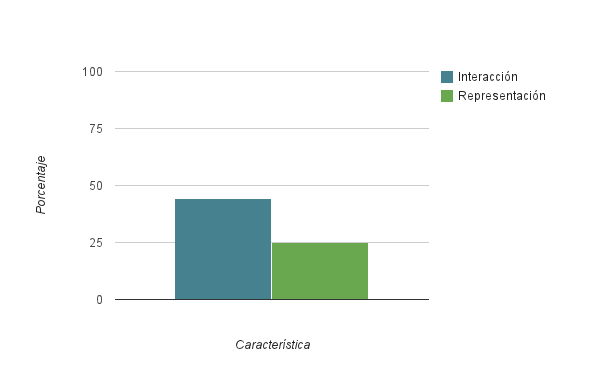
\includegraphics[scale=0.8]{resultados/imagenes/interfaz_disconformidad_caracteristica.png}
\caption{Disconformidad por característica}
\label{fig:interfaz_disconformidad_caracteristica}
\end{figure}

Además de estos datos, las grabaciones realizadas a las sesiones de los usuarios
se utilizan para medir el grado de facilidad de aprendizaje de la interfaz de
usuario. Con las variables y métricas descriptas en la
sección~\ref{sec:interfaz} agrupamos los datos en tres según las actividades que
puede realizar el usuario con la interfaz.

Estos tres grupos son los siguientes: 

\begin{itemize}
\item \textbf{Operación:} se refiere a las actividades que el usuario puede
    realizar utilizando el menú contextual que aparece sobre cada una de las
    herramientas que pueden ser empleadas en el procedimiento de enfermería que
    se le presente.
\item \textbf{Acción:} se refiere a las actividades que el usuario puede
    realizar seleccionando una opción en alguno de los dos menús principales que
    presenta la interfaz de la solución propuesta.
\item \textbf{Utilización:} se refiere a las actividades que el usuario puede
    realizar cuando tiene seleccionada una herramienta sin hacer uso de las
    opciones que ofrece el menú contextual.
\end{itemize}

Dados los tres grupo descriptos, la tabla~\ref{tab:interfaz_tiempo_actividades}
nos muestra el tiempo, en segundos, que le tomo a cada usuario realizar cada una
de las actividades la primera vez y el tiempo que les tomo en promedio las demás
veces, para cada una de los grupos de actividades.

\begin{table}[!hbt]
\centering
\begin{tabular}{|c|c|c|c|c|c|c|}
\hline
\rowcolor{gris} \textbf{Usuario/Actividad} & \multicolumn{2}{|c|}{\textbf{Operación}} & \multicolumn{2}{|c|}{\textbf{Acción}} & \multicolumn{2}{|c|}{\textbf{Utilización}}\\
\hline
\rowcolor{gris}  & Primera & Siguientes & Primera & Siguientes & Primera & Siguientes \\
\hline 1 & 8  & 2.25  & 3  & 9.14 & 11 & 3.0 \\
\hline 2 & 30 & 7.00  & 4  & 3.57 & 7  & 4.5 \\
\hline 3 & 5  & 2.25  & 5  & 1.86 & 1  & 1.0 \\
\hline 4 & 2  & 13.00 & 4  & 2.00 & 1  & 0.5 \\
\hline 5 & 18 & 2.75  & 6  & 4.43 & 6  & 3.0 \\
\hline 6 & 4  & 14.25 & 11 & 7.86 & 13 & 4.0 \\
\hline 7 & 5  & 8.00  & 4  & 4.71 & 20 & 2.5 \\
\hline 8 & 3  & 2.33  & 10 & 3.57 & 3  & 6.5 \\
\hline
\end{tabular}
\caption{Tiempo por actividades la primera vez y las siguientes veces que se realizo}
\label{tab:interfaz_tiempo_actividades}
\end{table}


De la tabla~\ref{tab:interfaz_tiempo_actividades} se obtienen dos resultados
importantes. El primero se puede observar en la
figura~\ref{fig:interfaz_tiempo_actividades} en donde se muestra el tiempo que
les tomo a los usuarios en promedio realizar las actividades la primera vez y
las demás veces. Se puede observar como en promedio el usuario aprende y en las
siguientes actividades similares demora menos tiempo para realizar las mismas.

\observacion{Hay que desarrollad mas la sección anterior}

\begin{figure}[hbt!]
\centering
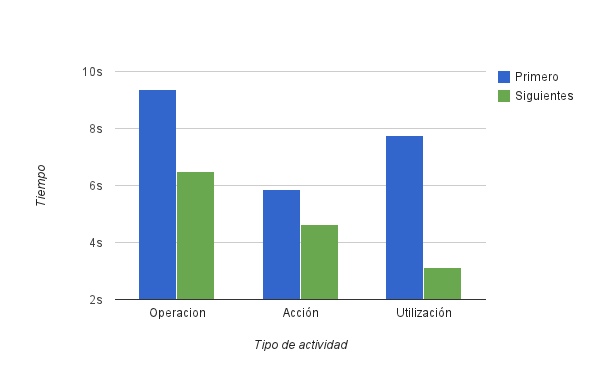
\includegraphics[scale=0.8]{resultados/imagenes/interfaz_tiempo_actividades.png}
\caption{Tiempo por tipo de actividad}
\label{fig:interfaz_tiempo_actividades}
\end{figure}

 
El segundo resultado se puede observar en el
gráfico~\ref{fig:interfaz_tiempo_total_actividades} que muestra el tiempo total
utilizado para realizar las diferentes actividades. Se puede apreciar que la
primera vez que se realizan las actividades se tardo 23 segundos, y las
siguientes veces 14.25 segundos. De esta manera, el tiempo empleado se redujo en
un $40\%$.

 
\begin{figure}[hbt!]
\centering
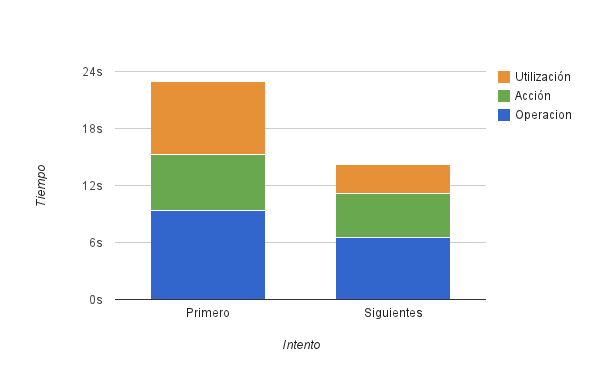
\includegraphics[scale=0.8]{resultados/imagenes/interfaz_tiempo_total_actividades.png}
\caption{Tiempo total por intento}
\label{fig:interfaz_tiempo_total_actividades}
\end{figure}
